\documentclass[a4paper,11pt]{article}

%\documentclass[a4paper,11pt,UTF8]{article} % For notes in Chinese
%\usepackage{ctex} % Used XeLaTeX with the "UTF8" unicode

%\usepackage[sc]{mathpazo} % Use the Palatino font
%\usepackage[T1]{fontenc} % Use 8-bit encoding that has 256 glyphs
%\linespread{1.15} % Line spacing - Palatino needs more space between lines
%\usepackage{microtype} % Slightly tweak font spacing for aesthetics

\usepackage[top=2cm,bottom=2.5cm,left=3cm,right=3cm]{geometry}
\usepackage{amsmath,amsfonts,amssymb,mathrsfs,graphicx,xcolor,bm}
\definecolor{myblue}{rgb}{0.18,0.19,0.57}
\definecolor{myred}{rgb}{0.75,0.00,0.00}
\usepackage[colorlinks, linkcolor=magenta, citecolor=blue, urlcolor=magenta]{hyperref}
\usepackage{titletoc}
\usepackage{authblk}
\usepackage{caption,lipsum}
\definecolor{lightgray}{gray}{0.98}

\begin{document}


\title{\Large\textbf{Paper of one column}}
\author{Ang Chen\thanks{chenang@outlook.com}} % if you have many authors, use the command "\author[1]{}, \author[2]{}, ...
% \affil{PBG group, Shanghai, China} %  "\affil[1]{}, \affil[2]{}, ...
\date{\today} %  "\date{}" means that you don't need date to appear; if you remove the command "\date{}", the date would appear, the same as the command "\date{\today}"


\maketitle

\section{Test}

\lipsum[1-2]

\begin{figure}[h]
\centering
% Requires \usepackage{graphicx}
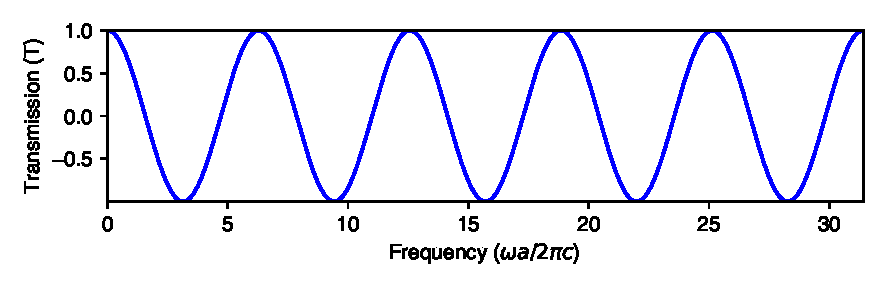
\includegraphics[scale=1]{../../figs/one_column_py.pdf} \\
\caption{\label{fig:from_python} Matplotlib.}
\end{figure}

\lipsum[3]

\begin{figure}[h]
\centering
% Requires \usepackage{graphicx}
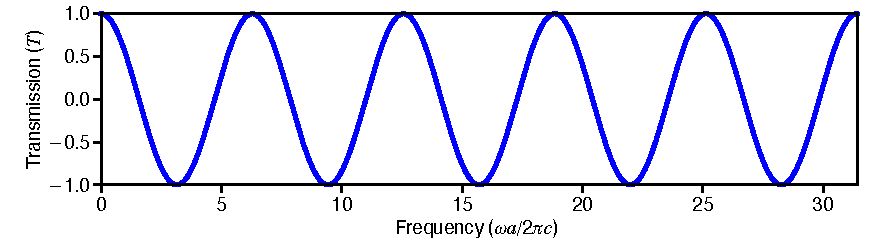
\includegraphics[scale=1]{../../figs/one_column_pressed.pdf} \\
\caption{\label{fig:pressed} Pressed.}
\end{figure}

\lipsum[4]







\end{document} 